\chapter{Implementation \TO}\label{Chapter:implementation-introduction}
This chapter will present the implementation of the \textit{Decomposition} project that was built around the algorithms described in Sections~\ref{Subsection:LU-decomposition-crout-method} and \ref{Subsection:LU-decomposition-numerical-method}. First, the \textit{TNL} library\footnote{TNL Library GitLab repository URL: \url{https://gitlab.com/tnl-project/tnl}} will be introduced briefly as it contains a structure that was paramount to the implementation of this project. Then, the description of the \textit{Decomposition} project itself will follow. Finally, the last section will present how the iterative algorithm, mentioned in Section~\ref{Subsection:LU-decomposition-numerical-method}, was fine-tuned for optimal performance using CUDA.

\section{TNL Library \TO}\label{Section:implementation-tnl-library}
The Template Numerical Library (TNL) is a collaborative, open-source project licensed under the MIT license. It aims to use modern programming paradigms combined with the computational power of parallel architectures to provide highly performant numerical solvers and simulations. In terms of parallel architectures, TNL supports both multi-core CPUs (using OpenMP\footnote{OpenMP website URL: \url{https://www.openmp.org/}}) and GPUs (as of July 2022 only CUDA-enabled Nvidia GPUs with compute capability 9.0 or higher \cite{Ednu6dyrkWKz1Bv2}). As TNL is written in C++ (with the exception of some helping Python/Bash scripts) it is designed to benefit from C++ templates and the advantages they bring. For example, the use of template specializations allows for minimal run-time overhead which makes execution of architecture-dependent code simple and fast \cite{Oberhuber20210210}. Further up-to-date information regarding TNL can be found on the project's website\footnote{TNL project website URL: \url{https://tnl-project.org/}}. \\
While TNL contains, among others, many different data structures. For the purpose of this project only the one used during development will be introduced.

\paragraph{Dense Matrix}\label{Paragraph:implementation-tnl-library-dense-matrix}
As mentioned at the end of Section~\ref{Subsection:LU-decomposition-numerical-method}, the goal of this project is to combine the parallel nature of CUDA-enabled Nvidia GPUs and the heavily parallelizable algorithm described in the same section (labeled as \textit{Iterative Crout method} for the purpose of this project). \\
Therefore, in order to store all matrices involved in the computation, an efficient, robust and intuitive data structure was required. While in terms of matrices TNL mainly revolves around sparse implementations (i.e. efficiently storing and performing operations with matrices that have more zero than non-zero elements), it also possesses the opposite: \textit{dense matrices}. As the name suggest, dense matrices are matrix structures densely populated with elements. In other words, a dense matrix stores every single element, regardless of its value (zeros and non-zeros are stored). In TNL, the class representing the dense matrix data structure is called \code{DenseMatrix} and it is located in the \code{TNL::Matrices} namespace. Similarly to the majority of classes representing matrices in TNL, it inherits from the \code{Matrix} class; the visualization of inheritance can be found in Figure~\ref{Figure:implementation-tnl-library-dense-matrix}.

\begin{figure}[h!]
	\centering
	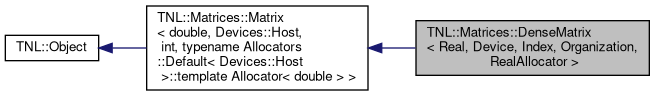
\includegraphics[width=\textwidth, keepaspectratio]{images/ch2/tnl_matrices_dense_matrix-inheritance.png}
	\caption{Inheritance diagram for the \code{TNL::Matrices::DenseMatrix} class. Taken from the \emph{Template Numerical Library Documentation} \cite{Ednu6dyrkWKz1Bv2}.}
	\label{Figure:implementation-tnl-library-dense-matrix}
\end{figure}

In the diagram shown in Figure~\ref{Figure:implementation-tnl-library-dense-matrix} the \code{DenseMatrix} class contains the following template parameters \cite{Ednu6dyrkWKz1Bv2}:

\begin{itemize}
	\item \code{Real} - Datatype of the matrix's elements, for example, \code{float} or \code{double} (default).
	\item \code{Device} - Type of device that the matrix structure is stored on. Its value can be either \code{TNL::Devices:Host} (default) or \code{TNL::Devices::Cuda}. The former indicates that the structure is stored in host memory, whereas the latter indicates that the data is stored in device memory. Furthermore, this parameter dictates which of the class's methods can be called and what device-dependent code should be executed.
	\item \code{Index} - Datatype of the matrix's index, for example, \code{short}, \code{int} (default), or \code{long}.
	\item \code{Organization} - Type of matrix element ordering. It can be either \code{RowMajorOrder} or \code{ColumnMajorOrder}. The former indicates that the elements of the matrix are stored in row-major order in a \code{DenseMatrix} instance's 1D array \code{values}, whereas the latter dictates that the elements are stored in the array in a column-major order. Implicitly, row-major order is used when the structure is allocated on the host and column-major order if it is allocated on the device.
	\item \code{RealAllocator} - Allocator for the matrix elements.
\end{itemize}

The \code{DenseMatrix} class contains an assortment of methods with varying functionalities - from the initialization of an entire matrix via arrays to per-element lambda functions and CUDA-tailored algorithms. In terms of this project, the most used methods were those that set and get elements, which can be done by using \code{setElement()} and \code{getElement()} respectively. Alternatively, for setting and getting elements, \code{DenseMatrix} possesses the overloaded operator: \code{operator()}, which allows the developer to write cleaner code that conveys its purpose more clearly. From the perspective of performance, both approaches are congruous as they take the same arguments and compute the index of the element in the instance's 1D array. Nonetheless, there is a difference between the two approaches: \code{operator()} has the \code{\_\_cuda\_callable\_\_} prefix, which specifies that it can be called from both host functions and CUDA kernels. However, this prefix comes with certain caveats:

\begin{itemize}
	\item Data allocated on the host can only be accessed by \code{operator()} from host functions.
	\item Data allocated on the device can only be accessed by \code{operator()} from the device, specifically, from CUDA kernels. For example, if an instance of \code{DenseMatrix} has \code{Device} set to \code{TNL::Devices::Cuda} and \code{operator()} would be used to access data from a host function, then the program would fail.
\end{itemize}

The limitations above are not present for the other approach (\code{setElement()} and \code{getElement()}). In other words, both \code{setElement()} and \code{getElement()} can be used from host functions and CUDA kernels, irrespective of where the \code{DenseMatrix} instance is allocated. However, this convenience has a pitfall: accessing data stored on the other device type. For example, let an instance of \code{DenseMatrix} be stored in device memory. Then, if it is accessed from a host function using \code{getElement()}, the procedure will be slow and only the value of the element will be returned. Listing~\ref{Listing:implementation-dense-matrix-getters-setters} shows an example of both approaches - including the caveats and pitfalls.

\begin{lstlisting}[caption={Code example showing the use of \code{setElement()}, and \code{operator()}; \code{getElement()} and getting a matrix element using \code{operator()} would be done similarly. The example requires the TNL library to already be installed. As mentioned in the code, the \code{setElements()} function will run correctly when evoked using the \code{TNL::Devices::Host} template parameter. However, if the \code{DenseMatrix} instance is allocated on the device, then the first setting of elements (using \code{setElement()}) will be slow due to the data transfer between the host and the device - each call will mean a unique data transfer. Furthermore, the second setting of elements (using \code{operator()}) will fail as \code{operator()} will be called from a host function on a \code{DenseMatrix} instance allocated on the device. For the second setter to work, it would need to be called from within a kernel. Taken from section \code{Tutorials/Matrices/DenseMatrices} in the \emph{Template Numerical Library Documentation} \cite{Ednu6dyrkWKz1Bv2}.},label={Listing:implementation-dense-matrix-getters-setters}]
#include <iostream>
#include <TNL/Matrices/DenseMatrix.h>
#include <TNL/Devices/Host.h>

template< typename Device >
void setElements()
{
	// Create an instance of 5x5 DenseMatrix
	TNL::Matrices::DenseMatrix< double, Device > matrix( 5, 5 );
	
	// Set elements of the main diagonal using setElement()
	for( int i = 0; i < 5; i++ )
		matrix.setElement( i, i, i );
	
	// Increment elements of the main diagonal using operator()
	for( int i = 0; i < 5; i++ )
		matrix( i, i ) += i;
}

int main( int argc, char* argv[] )
{
	// This example will run without any problems
	std::cout << "Set elements on host:" << std::endl;
	setElements< TNL::Devices::Host >();
	
#ifdef HAVE_CUDA
	// This example will fail on the second setting of elements
	std::cout << "Set elements on CUDA device:" << std::endl;
	setElements< TNL::Devices::Cuda >();
#endif
}
\end{lstlisting}

More detailed information on the structure's implementation can be found under \code{Namespaces/TNL/Matrices/DenseMatrix} in \emph{Template Numerical Library Documentation} \cite{Ednu6dyrkWKz1Bv2} and further examples of usage can be found under \code{Tutorials/Matrices/DenseMatrices}.



\section{Decomposition project \TO}\label{Section:implementation-decomposition-project}
Even though the \code{DenseMatrix} class from TNL is used in the Decomposition project - and a select few solvers are already implemented in TNL - it was decided to create a separate repository\footnote{\label{Footnote:decomposition-project-gitlab-url}Decomposition GitLab repository URL: \url{https://mmg-gitlab.fjfi.cvut.cz/gitlab/tnl/lu-decomposition}} in GitLab solely for this rendition of decomposition. Since the project is continually under development it is only available internally,
i.e. to users belonging to the TNL group on the Mathematical Modelling Group's\footnote{MMG main page URL: \url{https://geraldine.fjfi.cvut.cz/mmg/index.php}} GitLab page\footnote{TNL GitLab group URL: \url{https://mmg-gitlab.fjfi.cvut.cz/gitlab/tnl}}. \\
Although development was done outside of TNL, its structuring and building processes were adopted with minor changes to allow for easier familiarization and to keep the option of incorporating the Decomposition project into TNL open for the future. The compilation/installation of the project is done using the \code{install} Bash script that was adopted from TNL. The script itself serves as a wrapper for the \code{build} script that takes several building arguments, for example, the mandatory target parameter allows the user to choose to build one of the following:

\begin{itemize}
	\item \code{all} - compile the entire project including all other targets and the algorithm implementations.
	\item \code{benchmark} - compile the benchmark only.
	\item \code{tests} - compile the unit tests only.
\end{itemize}

Additionally, the \code{build} script provides optional parameters that can aid in compilation, for example:
\begin{itemize}
	\item \code{---install} - enables installation of the Decomposition project files into \code{\$HOME/.local/include}.
	\item \code{---cmake} - allows the user to supply the path to the CMake that is to be used for compilation.
	\item \code{---with-cuda-arch} - allows the user to specify the CUDA compute capability version to compile the project with. While there is an auto-detect feature for this parameter, the manual setting can be indispensable in some situations, for example, when running the benchmark on a computational cluster the compilation is usually done beforehand on a node that is not guaranteed to have a CUDA-enabled GPU. 
\end{itemize}

The full list of compilation options (\code{build} script usage) can be found in Attachment~\ref{Attachment:decomposition-project-build-script-parameters}. \\
The \code{build} script then calls CMake\footnote{CMake website URL: \url{https://cmake.org/}} which subsequently takes care of the build process using instructions from \code{CMakeLists.txt} files interspersed throughout the project. \\
The Decomposition project was written in \textit{C++} which was extended by \textit{CUDA} (GPU programming) and \textit{GoogleTest}\footnote{\label{Footnote:google-test}GoogleTest GitHub repository URL: \url{https://github.com/google/googletest}} (unit testing - approach adopted from TNL's matrix unit tests). Additionally, \textit{Python}\footnote{Python website URL: \url{https://www.python.org/}} and \textit{Bash}\footnote{Bash website URL: \url{https://www.gnu.org/software/bash/}} were used when adopting scripts from TNL, for example, a python script that creates tables and graphs in HTML from json files generated by the benchmark. \\
In this section, each part of the project's structure will be briefly described. First, unit tests will be detailed followed by the implementation of the Crout method (introduced in Section~\ref{Subsection:LU-decomposition-crout-method}), along with the Iterative Crout method (introduced in Section~\ref{Subsection:LU-decomposition-numerical-method}). Finally, the last part focuses on the benchmark implementation that aims to put into perspective the performance differences between the direct and iterative approach. \\
The ordering of topics follows the development process which was inspired by Test-driven development\footnote{Test-driven development Wikipedia page URL: \url{https://en.wikipedia.org/wiki/Test-driven_development}} (TDD). Specifically, the unit tests were written first; they were purposefully failing. Then, the implementation of the Crout method, along with the Iterative Crout method followed; this saw the unit tests passing. Finally, the benchmark was added as a feature at the end - without unit tests.

\subsection{Unit Tests \TO}
Despite the simplicity of this project - implementation of two short algorithms - quality assurance is still a key factor that aims to minimize erring development. Not counting manual verification of functionalities, unit tests are the most basic form of quality assurance. They allow for continual development with near-instant feedback on any changes in the implementation. \\
As mentioned before, GoogleTest\footref{Footnote:google-test} was chosen as the testing framework. The main reasons behind this choice were:

\begin{itemize}
	\item GoogleTest was used successfully to implemented unit tests in TNL.
	\item GoogleTest has the ability to run tests of a test suite across class instances with different hard-set template parameter values.
	\item GoogleTest is simple to use and can be easily integrated with the Decomposition project.
	\item GoogleTest fully supports C++ and is still actively being developed (roughly at least one merged pull request a week as of July 2022).
\end{itemize}

As the testing infrastructure was mostly adopted from TNL (detailed in Section 3.1 of the author's bachelor thesis \textit{Formats for storage of sparse matrices on GPU} \cite{Cejka2020}) it will only be described briefly.

\par For each algorithm (Crout method and Iterative Crout method) a suite of unit tests was written. The aim of the tests was to verify that a matrix was decomposed within some reasonable error range which was obtained by comparing the decomposition result to either existing solutions or solutions computed by programs, such as MATLAB\footnote{MATLAB website URL: \url{https://www.mathworks.com/products/matlab.html}}. Examples of tests are:

\begin{itemize}
	\item \code{test\_CroutMethod2x2MatrixDecompose< MatrixType >()} - Test that the algorithm will decompose a 2x2 matrix correctly. The decomposition of a small matrix is likely to produce its exact solution, thus, tests where a such a matrix is decomposed can have zero tolerance when it comes to checking for errors in computation.
	\item \code{test\_CroutMethod38x38MatrixDecompose< MatrixType >()} - Test that the algorithm will decompose a 38x38 matrix correctly with some tolerance. The tolerance for solutions is required as the larger the dimensions, the more prone to differences the solutions are. This erring behavior is due to the limited accuracy of double and single precision when compared to, for example, MATLAB.
	\item \code{test\_CroutMethod10x10DecomposeSingularMatrixShouldFail< MatrixType >()} - Test that the algorithm will fail to decompose a 10x10 singular matrix. The execution of the program will fail as such a matrix cannot be decomposed without a permutation matrix which is not in the scope of this project.
\end{itemize}

In the examples of tests above, the \code{MatrixType} template parameter represents an instance of the \code{DenseMatrix} class from the set of instances which can be seen in Listing~\ref{Listing:implementation-decomposition-project-unit-tests-instances-set}. Additionally, Listing~\ref{Listing:implementation-decomposition-project-unit-tests-2x2-matrix-decomposition-test} shows the implementation of the 2x2 matrix test mentioned above in the list of examples and also in Listing~\ref{Listing:implementation-decomposition-project-unit-tests-instances-set}.

\begin{lstlisting}[caption={Implementation of the set of \code{DenseMatrix} instances and one test using GoogleTest. The unit tests are all run for each instance. The test suite is tied to the set of instances using \code{TYPED\_TEST\_SUITE} and each test is added to the test suite using the declaration \code{TYPED\_TEST}. Taken from the Decomposition project repository on GitLab\protect\footref{Footnote:decomposition-project-gitlab-url}.},label={Listing:implementation-decomposition-project-unit-tests-instances-set}]
template< typename Matrix >
class ILUCroutMethodTest : public ::testing::Test
{
	protected:
		using MatrixType = Matrix;
};

using MatrixTypes = ::testing::Types<
TNL::Matrices::DenseMatrix< float,  TNL::Devices::Host, short >,
TNL::Matrices::DenseMatrix< double, TNL::Devices::Host, short >,
TNL::Matrices::DenseMatrix< float,  TNL::Devices::Host, int   >,
TNL::Matrices::DenseMatrix< double, TNL::Devices::Host, int   >,
TNL::Matrices::DenseMatrix< float,  TNL::Devices::Host, long  >,
TNL::Matrices::DenseMatrix< double, TNL::Devices::Host, long  >
#ifdef HAVE_CUDA
,TNL::Matrices::DenseMatrix< float, TNL::Devices::Cuda, short, TNL::Algorithms::Segments::RowMajorOrder >,
TNL::Matrices::DenseMatrix< double, TNL::Devices::Cuda, short, TNL::Algorithms::Segments::RowMajorOrder >,
TNL::Matrices::DenseMatrix< float,  TNL::Devices::Cuda, int,   TNL::Algorithms::Segments::RowMajorOrder >,
TNL::Matrices::DenseMatrix< double, TNL::Devices::Cuda, int,   TNL::Algorithms::Segments::RowMajorOrder >,
TNL::Matrices::DenseMatrix< float,  TNL::Devices::Cuda, long,  TNL::Algorithms::Segments::RowMajorOrder >,
TNL::Matrices::DenseMatrix< double, TNL::Devices::Cuda, long,  TNL::Algorithms::Segments::RowMajorOrder >
#endif
>;

TYPED_TEST_SUITE( ILUCroutMethodTest, MatrixTypes );

TYPED_TEST( ILUCroutMethodTest, croutMethod2x2MatrixDecomposeTest )
{
	using MatrixType = typename TestFixture::MatrixType;
	test_CroutMethod2x2MatrixDecompose< MatrixType >();
}
\end{lstlisting}

\begin{lstlisting}[caption={Implementation of the test where a 2x2 \code{DenseMatrix} instance is decomposed. As mentioned before, the matrix decomposed in this test is small and therefore the decomposed $ \mathbb{L} $ and $ \mathbb{U} $ matrices are expected to be exact solutions rather than within some range of the exact solution. Taken from the Decomposition project repository on GitLab\protect\footref{Footnote:decomposition-project-gitlab-url}.},label={Listing:implementation-decomposition-project-unit-tests-2x2-matrix-decomposition-test}]
template< typename Matrix >
void test_CroutMethod2x2MatrixDecompose()
{
	const Matrix A( {
		{ 4, 24 },
		{ 2, 15 }
	} );
	
	Matrix L, U;
	L.setLike( A );
	U.setLike( A );
	
	Decomposition::LU::CroutMethodIterative::decompose( A, L, U );
	
	EXPECT_EQ( L.getElement( 0, 0 ),  4.0 );
	EXPECT_EQ( L.getElement( 0, 1 ),  0.0 );
	EXPECT_EQ( L.getElement( 1, 0 ),  2.0 );
	EXPECT_EQ( L.getElement( 1, 1 ),  3.0 );

	EXPECT_EQ( U.getElement( 0, 0 ),  1.0 );
	EXPECT_EQ( U.getElement( 0, 1 ),  6.0 );
	EXPECT_EQ( U.getElement( 1, 0 ),  0.0 );
	EXPECT_EQ( U.getElement( 1, 1 ),  1.0 );
}

\end{lstlisting}

Since the unit tests are run with every compilation of the algorithms they had to be lightweight. Thus, matrix dimensions of tested matrices ranged from 2x2 to only 38x38 and included the following: 2x2, 3x3, 4x4, 10x10, 19x19 and 38x38. The larger dimensions - from 10x10 - were chosen to test a specific part of the Iterative Crout method's implementation on the GPU: matrix convergence by sections (detailed in Section~\ref{Subsection:implementation-decomposition-project-lu-decomposition}).


\subsection{LU Decomposition \TO}\label{Subsection:implementation-decomposition-project-lu-decomposition}
The core of the Decomposition project is made up of the Crout method and the Iterative Crout method, detailed in Section~\ref{Subsection:LU-decomposition-crout-method} and Section~\ref{Subsection:LU-decomposition-numerical-method} respectively. This part contains a description of their implementations. First, it is necessary to introduce a memory-saving concept used in this project. Then, the requirements for the implementations will be presented and, finally, the description of the implementations of the individual algorithms will follow.

\paragraph{Memory-saving concept} Whenever LU decomposition was mentioned in the previous chapters and sections, it was presented as decomposing matrix $ \mathbb{A} $ into matrices $ \mathbb{L} $ and $ \mathbb{U} $. However, since \code{DenseMatrix} stores every element of a matrix and the upper triangle of $ \mathbb{L} $ and the lower triangle of $ \mathbb{U} $ are zeros, then only half of the elements stored in the two matrices are used during decomposition. Therefore, to avoid using memory unnecessarily, another approach was used in alongside the original: store $ \mathbb{L} $ and $ \mathbb{U} $ into a single matrix $ \mathbb{Z} $. The lower triangle of matrix $ \mathbb{Z} $ (including the main diagonal) would house the elements of $ \mathbb{L} $ and the upper triangle (excluding the 1s on the main diagonal) would be made up of elements from $ \mathbb{U} $. \\
While this approach uses less memory, it has some drawbacks:

\begin{itemize}
	\item it is not aligned with the convention of LU decomposition to return two matrices; and
	\item it does not store the 1s found on the main diagonal of $ \mathbb{U} $.
\end{itemize}

Thus, in order for the decomposed solution to be used it may be required to extract matrices $ \mathbb{L} $ and $ \mathbb{U} $ from matrix $ \mathbb{Z} $ - this step is not implemented in the Decomposition project currently and is up to the user to handle it for now. \\
Nevertheless, to save memory, in this project every decomposing method is written in two variants:

\begin{enumerate}
	\item Decompose matrix $ \mathbb{A} $ into matrices $ \mathbb{L} $ and $ \mathbb{U} $.
	\item Decompose matrix $ \mathbb{A} $ into matrix $ \mathbb{Z} $ which contains elements of $ \mathbb{L} $ and $ \mathbb{U} $ - except for their zero-filled triangles and the main diagonal of $ \mathbb{U} $.
\end{enumerate}

\paragraph{Implementation requirements}\label{Paragraph:implementation-decomposition-project-lu-decomposition-implementation-requirements} To put the algorithms mentioned earlier into context of the project's tasks, the tasks requiring some sort of implementation were the following:

\begin{enumerate}
	\item Implement a parallel version of LU decomposition in CUDA for GPUs.
	\item Measure the acceleration of the GPU version of the LU decomposition against the CPU version.
\end{enumerate}

In other words, this means implementing the following:

\begin{enumerate}
	\item Crout method for the CPU detailed in Section~\ref{Subsection:LU-decomposition-crout-method}.
	\item Iterative Crout method for the GPU detailed in Section~\ref{Subsection:LU-decomposition-numerical-method}.
\end{enumerate}

As mentioned at the beginning of this Section, the process of development was inspired by TDD. Thus, once unit tests were implemented and successfully failing, the implementation of the algorithms began.

\paragraph{Crout method}\label{Paragraph:implementation-decomposition-project-lu-decomposition-crout-method}
The Crout method - as described in Section~\ref{Subsection:LU-decomposition-crout-method} - was implemented only for the CPU as implementing it on the GPU would not bring any interesting results since it is a sequential algorithm. \\
Since the implementation of the Crout method in the Decomposition project differs slightly from the pseudo-code shown in Listing~\ref{Listing:LU-decomposition-crout-method-pseudocode}, the code is shown only in Attachment~\ref{Attachment:crout-method-implementation-CPU}. \\
One of the noticeable differences between the pseudo-code from Listing~\ref{Listing:LU-decomposition-crout-method-pseudocode} and the implementations is that the lines where the elements on the main diagonal of $ \mathbb{U} $ are all set to 1s are not present in the latter. They were removed as it was observed that they were not needed since the algorithm would compute them regardless.

\paragraph{Iterative Crout method}\label{Paragraph:implementation-decomposition-project-lu-decomposition-iterative-crout-method}
According to the requirements mentioned above, the Iterative Crout method was to be implemented only on the GPU, however, in order to verify the correctness of the results its first version was also implemented on the CPU. \\
The CPU version served purely as a means to verify that the GPU version did not exhibit unexpected behaviors due to parallelism, for example, race conditions. In this instance, a race condition refers to a scenario where one thread would overwrite a value before another thread would read the old value. After a brief comparison of results produced by the CPU and GPU versions on a set of matrices no differences were found. Thus, even though originally it was planned for the CPU version to mirror the GPU version and have it continually verify the results, this approach was abandoned due to the large computational time required for the CPU version to complete. In summary, the CPU version only mirrors the initial GPU version and was not developed further. \\
The GPU version of the Iterative Crout method went through various optimizations during development - the different concepts are detailed in Section~\ref{Section:implementation-optimization}. This section will only present the latest - and for now final - GPU version that uses matrix $ \mathbb{Z} $. \\
The GPU implementation can be split into two parts:

\begin{enumerate}
	\item Convergence by sections.
	\item Convergence of a single section using the Iterative Crout method detailed in Section~\ref{Subsection:LU-decomposition-numerical-method}.
\end{enumerate}

\subparagraph{Convergence by sections}\label{Subparagraph:implementation-decomposition-project-lu-decomposition-iterative-crout-method-convergence-by-sections}
This part leverages advantages from both the sequential and parallel versions of the Crout method in order to optimize the entire procedure. \\
Similarly to the Iterative algorithm detailed in Section~\ref{Subsection:LU-decomposition-numerical-method}, the \textit{convergence by sections} concept begins by providing an initial estimate of matrix $ \mathbb{Z} $, for example, $ \mathbb{Z} = \mathbb{A}$. Then, $ \mathbb{Z} $ is divided into equally-sized sub-matrices (in this project, the sub-matrices are called \textit{sections} and are labeled with $ _{sub} $, for example, $ \mathbb{Z}_{sub} $). Then, beginning in the top-left corner, the sections are sequentially converged (equivalent to a sub-matrix being decomposed) using the Iterative Crout method algorithm described in Section~\ref{Subsection:LU-decomposition-numerical-method}. The order in which sections are converged is crucial to achieving near-optimal execution times; it is shown in Figure~\ref{Figure:implementation-decomposition-project-lu-decomposition-order-of-convergence-of-sections}.

\begin{figure}[h!]
	\vspace{0.8cm}					  % Add space above figure to make room for the 's' label above the matrix
	\setlength{\arraycolsep}{24pt}    % Larger gap between columns
	\renewcommand{\arraystretch}{3.6} % Larger gap between rows
	\[\begin{bNiceArray}{cccc}[margin=26pt, create-medium-nodes]
		0 & 1 & 2 & 3 \\
		1 & 4 & 5 & 6 \\
		2 & 5 & 7 & 8 \\
		3 & 6 & 8 & 9 \\
		\CodeAfter
		\begin{tikzpicture}
			\draw[decorate, decoration=brace, transform canvas={xshift=5.75em}, thick] (row-1-|col-4) -- node[right=2pt] {\large $s$} (row-2-|col-4);
			\draw[decorate, decoration=brace, transform canvas={yshift=0.5em}, thick] (row-1-|col-4) -- node[above=2pt] {\large $s$} (row-1-|col-5);
			\foreach \i in {2,...,4}
			{
				\draw[densely dotted] (row-\i-|col-1) -- (row-\i-|col-5);
				\draw[densely dotted] (row-1-|col-\i) -- (row-5-|col-\i);
			}
		\end{tikzpicture}
	\end{bNiceArray}\]
	\caption{Visualization of matrix $ \mathbb{Z} $ divided into sections of size $ s\times s $. The order in which sections are converged is denoted by the number in each section. First, the upper-left-most section (section '$ 0 $') is converged, then, the sections below and to the right of it (sections labeled with a '$ 1 $') are converged in parallel. Then, certain sections to the right and below of each section '$ 1 $' (sections labeled with '$ 2 $') are converged in parallel etc.}
	\label{Figure:implementation-decomposition-project-lu-decomposition-order-of-convergence-of-sections}
\end{figure}

The order of convergence of sections is derived from the fact that a single element in $ \mathbb{Z} $, for example, $ z_{ij} $ (where $ i,j \in \widehat{n} $), is computed using only some elements above and to the left of it. Specifically, only $ 2x $ (where $ x = \min(i, j) $) elements will be used, i.e. in row $ i $ only columns $ \left[0, x\right] $ and in column $ j $ only rows $ \left[0, x\right] $. This means that the quality of an element's value greatly depends on the quality of the elements used to compute it (quality refers to how close an element is to its final (converged) value in a given iteration). The visualization of what elements are used to compute a single element $ z_{ij} $ is shown in Figure~\ref{Figure:implementation-decomposition-project-lu-decomposition-element-dependance}.

\begin{figure}[h!]
	\centering
	\begin{subfigure}{.5\textwidth}
		\centering
		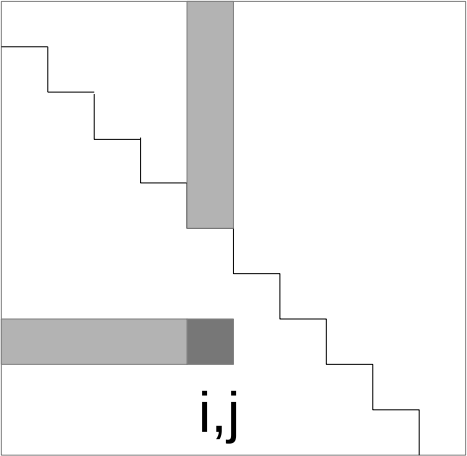
\includegraphics[width=.8\textwidth, keepaspectratio]{images/ch2/LU_decomposition_crout_method_visualization_elements_used_simple_lower.png}
		\label{Figure:implementation-decomposition-project-lu-decomposition-element-dependance-lower}
	\end{subfigure}%
	\begin{subfigure}{.5\textwidth}
		\centering
		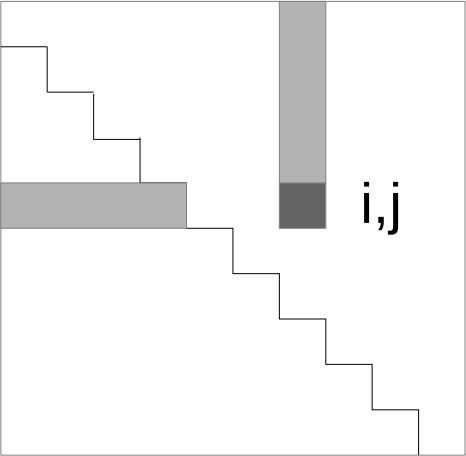
\includegraphics[width=.8\textwidth, keepaspectratio]{images/ch2/LU_decomposition_crout_method_visualization_elements_used_simple_upper.png}
		\label{Figure:implementation-decomposition-project-lu-decomposition-element-dependance-upper}
	\end{subfigure}
	\caption{Examples showing the elements used (shaded regions) to calculate an element at row $ i $ and column $ j $ (dark square). As described earlier, only elements with indices in the interval $ \left[0, \min(i, j)\right] $ are used in the element's row and column. Taken from E. Chow's and A. Patel's \emph{Fine-Grained Parallel Incomplete LU Factorization} \cite{Chow2015}.}
	\label{Figure:implementation-decomposition-project-lu-decomposition-element-dependance}
\end{figure}

The implementation of the Iterative Crout method for the GPU using matrix $ \mathbb{Z} $ is shown in Listing~\ref{Listing:implementation-decomposition-project-lu-decomposition-iterative-crout-method-convergence-by-sections}. The listing does not contain the decomposition kernel itself as it is shown later in Listing~\ref{Listing:implementation-decomposition-project-lu-decomposition-iterative-crout-method-convergence-of-single-section} in \textit{\nameref{Subparagraph:implementation-decomposition-project-lu-decomposition-iterative-crout-method-convergence-of-single-section}}.

\begin{lstlisting}[caption={GPU implementation of the Iterative Crout method. Some code has been omitted as it is not important for the description, for example, checking if the input matrix is square. Overall, the code performs the following: initialization of variables (including CUDA grid specifications, page-locked host memory, streams, etc.), then the entire matrix $ \mathbb{A} $ is decomposed using the \textit{Convergence by sections} concept. The constant \code{BLOCK\_SIZE} dictates how many threads are present in a single thread block. The \code{converged\_host} variable is purposefully initialized using page-locked host memory as its value is copied between the host and device in every iteration of the do-while loop. Thus, as described in \textit{\nameref{Paragraph:CUDA-memory-management-page-locked-host-memory}} in Section~\ref{Paragraph:CUDA-memory-management-page-locked-host-memory}, the higher bandwidth provided can help reduce the overall time spent copying during computation. Taken from the Decomposition project repository on GitLab\protect\footref{Footnote:decomposition-project-gitlab-url}.},label={Listing:implementation-decomposition-project-lu-decomposition-iterative-crout-method-convergence-by-sections},escapechar=@]
template< typename Matrix1,	typename Matrix2 >
void CroutMethodIterative::decompose( Matrix1& A, Matrix2& Z )
{
	using Real   = typename Matrix1::RealType;
	using Device = typename Matrix1::DeviceType;
	using Index  = typename Matrix1::IndexType;
	
	Index num_rows = A.getRows();
	Index num_cols = A.getColumns();
	
	Matrix2 Znew;
	Znew.setLike( Z );
	Z = A;
	bool converged = true;
	Real tolerance = 0;
	
	// Compute the size of a section
	Index sectionSize = min( max( num_cols / 10, (Index)256 ), (Index)1024 );
	sectionSize = ( sectionSize + BLOCK_SIZE - 1 ) / BLOCK_SIZE * BLOCK_SIZE;
	
	// Determine the number of blocks based on the section size
	Index blocks = sectionSize / BLOCK_SIZE;
	dim3 threadsPerBlock( BLOCK_SIZE, BLOCK_SIZE );
	dim3 blocksPerGrid( blocks, blocks );
	
	// Copy required data to the GPU
	Matrix1* matrixA_kernel     = TNL::Cuda::passToDevice( A );
	Matrix2* matrixZ_kernel     = TNL::Cuda::passToDevice( Z );
	Matrix2* matrixZnew_kernel  = TNL::Cuda::passToDevice( Znew );
	bool*    converged_kernel   = TNL::Cuda::passToDevice( converged );
	Real*    tolerance_kernel   = TNL::Cuda::passToDevice( tolerance );
	
	// Initialize the converged switch to page-locked host memory
	bool* converged_host = NULL;
	cudaMallocHost( (void **) &converged_host, sizeof(bool) );
	
	// Allocate and initialize an array of 2 stream handles
	int nstreams = 2;
	cudaStream_t *streams = (cudaStream_t *)malloc(nstreams * sizeof(cudaStream_t));
	for (int i = 0; i < nstreams; i++) {
		cudaStreamCreate(&(streams[i]));
	}
	
	// Initialize variables for keeping track of where the main diagonal section begins and ends
	Index diag_start, diag_end, sStart, sEnd;
	
	// Converge by sections
	for( diag_start = 0, diag_end = min( num_cols, sectionSize ); diag_start < diag_end; diag_start += sectionSize, diag_end = min( num_cols, diag_end + sectionSize) ) {
		// Converge the diagonal section first using the Default stream
		do {
			*converged_host = true;
			cudaMemcpy( converged_kernel, converged_host, sizeof(bool), cudaMemcpyHostToDevice );
			
			DecomposeKernel< Real, Index ><<< blocksPerGrid, threadsPerBlock >>>( matrixA_kernel, matrixZ_kernel, matrixZnew_kernel, diag_start, diag_end, diag_start, diag_end, tolerance_kernel, converged_kernel );
			
			// Synchronize after execution of kernel before copying value of converged
			cudaDeviceSynchronize();@\label{Line:decompose-method-cudaDeviceSynchronize-1}@
			cudaMemcpy( converged_host, converged_kernel, sizeof(bool), cudaMemcpyDeviceToHost );
		} while( !*converged_host );
		
		// Converge sections below and to the right of the main diagonal section using the two streams
		for( sStart = diag_end, sEnd = min( num_cols, diag_end + sectionSize );	sStart < sEnd;	sStart += sectionSize, sEnd = min( num_cols, sEnd + sectionSize ) ) {
			do {
				*converged_host = true;
				cudaMemcpy( converged_kernel, converged_host, sizeof(bool), cudaMemcpyHostToDevice );
				
				// Run Stream 1: iterate columns - rows should stay the same
				DecomposeKernel< Real, Index ><<< blocksPerGrid, threadsPerBlock, 0, streams[0] >>>( matrixA_kernel, matrixZ_kernel, matrixZnew_kernel, sStart, sEnd, diag_start, diag_end, tolerance_kernel, converged_kernel );
				
				// Run Stream 2: iterate rows - columns should stay the same
				DecomposeKernel< Real, Index ><<< blocksPerGrid, threadsPerBlock, 0, streams[1] >>>( matrixA_kernel, matrixZ_kernel, matrixZnew_kernel, diag_start, diag_end, sStart, sEnd, tolerance_kernel, converged_kernel );
				
				// Synchronize after execution of kernels before copying value of converged
				cudaDeviceSynchronize();@\label{Line:decompose-method-cudaDeviceSynchronize-2}@
				cudaMemcpy( converged_host, converged_kernel, sizeof(bool), cudaMemcpyDeviceToHost );
			} while( !*converged_host );
		}
	}
}
\end{lstlisting}

One of the first performance-determining aspects shown in Listing~\ref{Listing:implementation-decomposition-project-lu-decomposition-iterative-crout-method-convergence-by-sections} is the size of a section (\code{sectionSize} or $ s $). It affects both the speed of computation and the accuracy of results (detailed further in Chapter~\ref{Chapter:benchmark-results}). Specifically, the phrase "\textit{accuracy of results}" refers to how much the matrix resulting from $ \mathbb{L}\cdot\mathbb{U} $ differs from the original input matrix $ \mathbb{A} $. How the size of a section is calculated changed many times throughout development. Initially, the size of a section is set to $ 1/10 $ of the dimensions of $ \mathbb{Z} $, however, this value must be within the interval $ \left[256, 1024\right] $. If it is outside of this interval, then the size is set to the interval's closest endpoint (256 or 1024). Then, its value is rounded to the nearest multiple of \code{BLOCK\_SIZE} (8, 16, or 32) that is larger than the original \code{sectionSize} due to CUDA-related reasons described later in \textit{\nameref{Subparagraph:implementation-decomposition-project-lu-decomposition-iterative-crout-method-convergence-of-single-section}}. \\
In Figure~\ref{Figure:implementation-decomposition-project-lu-decomposition-order-of-convergence-of-sections} it can be seen that some sections are converged in parallel. In general, a section can be converged optimally only if specific sections above and to the left of it are already converged. The specific sections that the to-be-converged section depends are the same as the elements required to converge a specific element quickly. In order to imagine this better, the dark square in Figure~\ref{Figure:implementation-decomposition-project-lu-decomposition-element-dependance} can be considered as the to-be-converged section and the shaded regions can be considered as the sections that must be converged before it. It is noteworthy that the general concept - how a section can be converged optimally - allows for more than 2 sections can be converging simultaneously. This and any other potential performance improvements are detailed in Section~\ref{Section:implementation-optimization}. \\
As can be seen in Listing~\ref{Listing:implementation-decomposition-project-lu-decomposition-iterative-crout-method-convergence-by-sections} each section is converged using a decomposition kernel. Since each kernel is launched on a grid of blocks that are made up of threads, then each section is converged using a grid. Thus, in order to facilitate parallel convergence of sections, CUDA streams (detailed in Section~\ref{Subsubsection:CUDA-asynchronous-concurrent-execution-concurrent-streams}) were used. Specifically, sections that encompass the main diagonal (main diagonal sections) are converged using the default stream and sections converged in parallel were each given a separate stream, i.e. two streams are created and each is used to converge one of the parallel sections. For example - using the numbering of sections from Figure~\ref{Figure:implementation-decomposition-project-lu-decomposition-order-of-convergence-of-sections} - first, section '$ 0 $' is converged using the default stream. Then, sections labeled with a '$ 1 $' are converged - each using a different stream. Following that, sections labeled with a '$ 2 $' are converged - each using a different stream - and so on until sections labeled with a '$ 3 $'. Then section '$ 4 $' is converged, again using the default stream. \\
In summary, converging the input matrix by sections is faster than converging all of it at once since its elements - especially those in the lower-right corner - will have higher quality elements available for the computation of their value. For example, let $ z_{ij} $ (located in the lower-right corner of $ \mathbb{Z} $) be the currently computed element. If the entire matrix $ \mathbb{Z} $ is being converged at once and if it is a large matrix, then, since elements in the first few rows and columns (excluding the 1st row and column as their values are taken directly from $ \mathbb{A} $ and not altered further) are highly inaccurate they will cooperatively produce even less accurate elements in the later rows and columns - a snowball effect of low quality elements. Thus, during the first few iterations $ z_{ij} $ will be calculated using low quality elements and it will be far from its final converged value. Slowly, through multiple iterations the quality of elements will increase row-by-row and column-by-column which will in turn slowly converge $ z_{ij} $. Thus, when converging the entire matrix simultaneously, computing elements found further in the matrix (elements near and in the lower-right corner of the matrix) is a waste of resources and time. Ultimately, this makes convergence by sections more optimal.

\subparagraph{Convergence of a single section}\label{Subparagraph:implementation-decomposition-project-lu-decomposition-iterative-crout-method-convergence-of-single-section}
While the previous part detailed how an entire matrix is converged by sections, this part describes how a single section is converged. A single section denotes a $ s\times s $ sub-matrix of matrix $ \mathbb{Z} $ that is labeled $ \mathbb{Z}_{sub} $. Since the sub-matrix (section) is not being decomposed itself as a matrix, rather this part of matrix $ \mathbb{Z} $ is being decomposed, then, the phrase "\textit{single section is converged}" is befitting. In technical terms this means providing a series of inputs (sub-matrices, indexes, tolerance values, etc.) to a kernel that is executed on the device. First, for the explanation of the decomposition kernel, it is necessary to slightly alter the algorithm from Section~\ref{Subsection:LU-decomposition-numerical-method} - using matrix $ \mathbb{Z} $ instead of $ \mathbb{L} $ and $ \mathbb{U} $ - to the perspective of a section:

\begin{enumerate}
	\item Given input matrices $ \mathbb{A} $ and $ \mathbb{Z}^t $ calculate the next iteration of a specific sub-matrix: $ \mathbb{Z}^{t+1}_{sub} $:
		\begin{align}
			z_{ij}^{t+1} &= a_{ij} - \sum_{k=1}^{j-1}z_{ik}^{t}z_{kj}^{t}                                                              &\quad i \geq j \nonumber\,, \\
			z_{ij}^{t+1} &= \frac{1}{z_{ii}^{t}} \left ( z_{ij} - \sum_{k=1}^{i-1}z_{ik}^{t}z_{kj}^{t} \right ) &\quad i < j \nonumber\,.\\
		\end{align}
	\item Check if the section has converged according to the tolerance rule: $ \left | \mathbb{Z}^{t+1}_{sub} - \mathbb{Z}^{t}_{sub} \right | > tol $ (where $ tol $ is some hard-set value, for example, $ 0.0001 $). If the tolerance rule has not passed, then go back to step 2.
	\item If the tolerance rule has passed, then the algorithm has arrived to an approximate solution of a sub-matrix in $ \mathbb{L}\mathbb{U} $ (stored in $ \mathbb{Z} $).
\end{enumerate}

Note that the value of the $ tol $ parameter is another important factor that determines the performance (speed of execution and accuracy of results). If the value of the parameter is too high, for example, $ 1.5 $ then the algorithm will converge faster, however, the matrix resulting from $ \mathbb{L}\mathbb{U} $ will differ more significantly from $ \mathbb{A} $, i.e. the decomposition will be inaccurate. On the other hand, the closer the tolerance value is to zero, the more accurate the results will be, however, it will take longer for the algorithm to converge. This parameter went through many changes, before finally settling to $ 0.0 $. The reasons behind this decision were the following:

\begin{itemize}
	\item \textit{\nameref{Subparagraph:implementation-decomposition-project-lu-decomposition-iterative-crout-method-convergence-by-sections}} allows for greater granularity as the quality of each $ s \times s $ section depends on the quality of specific sections that were converged before it. Thus, setting the tolerance parameter to zero means that the elements of a section are computed using elements that are as accurate as possible.
	\item Testing the solution on a set of matrices that comprised of 61 sparse, dense, small and large matrices revealed that the difference in performance when setting the tolerance value near zero (for example, $ 0.0001 $) and just zero was negligible. However, the accuracy of results when $ tol = 0.0 $ was significantly higher - detailed further in Section~\ref{Section:implementation-optimization} and Chapter~\ref{Chapter:benchmark-results}.
	\item The testing further revealed that the accuracy of results can decrease if the dimensions of the input matrix increase. Thus, it was decided that even though speed of convergence is important, it loses meaning if the produced results are unusable.
\end{itemize}

The implementation of the decomposition kernel using matrix $ \mathbb{Z} $ is shown in Listing~\ref{Listing:implementation-decomposition-project-lu-decomposition-iterative-crout-method-convergence-of-single-section}.

\begin{lstlisting}[caption={The constant \code{BLOCK\_SIZE} is by default hard-coded to be equal to 8 in the \code{CroutMethodIterative} header file using the \code{\#define} macro. The kernel takes matrices $ \mathbb{A} $, $ \mathbb{Z} $ (iteration $ t $ of $ \mathbb{Z} $), and $ \mathbb{Z}_{new} $ (iteration $ t+1 $ of $ \mathbb{Z} $) as input parameters, and uses other input variables to offset the threads in the grid so that only a specific section of $ \mathbb{Z} $ is computed. Note that the kernel is not part of the \code{CroutMethodIteartive} class since kernels cannot be members of a class - as mentioned in \textit{\nameref{Paragraph:CUDA-C++-extensions-outer-kernel-extensions-function-extensions}} in Section~\ref{Paragraph:CUDA-C++-extensions-outer-kernel-extensions-function-extensions} - however, it is located in the same file that it is called from. Taken from the Decomposition project repository on GitLab\protect\footref{Footnote:decomposition-project-gitlab-url}.},label={Listing:implementation-decomposition-project-lu-decomposition-iterative-crout-method-convergence-of-single-section},escapechar=@]
template< typename Real, typename Index, typename Matrix1, typename Matrix2 >
__global__ void DecomposeKernel( const Matrix1* _A, Matrix2* _Z, Matrix2* _Znew, const Index col_sStart, const Index col_sEnd, const Index row_sStart, const Index row_sEnd, const Real* tolerance, bool* converged )
{
	auto& A = *_A; auto& Z = *_Z; auto& Znew = *_Znew;
	
	// Get a thread's sub-matrix ID that is offset to become a global ID of Z
	Index row = blockIdx.y * blockDim.y + threadIdx.y + row_sStart;
	Index col = blockIdx.x * blockDim.x + threadIdx.x + col_sStart;
	
	Index tx = threadIdx.x;
	Index ty = threadIdx.y;
	Real sum = 0;
	
	// Set overreaching thread ID to the closest edge of the matrix's dimensions
	Index max_col = col_sEnd - 1;
	Index max_row = row_sEnd - 1;
	Index new_row = min( row, max_row );
	Index new_col = min( col, max_col );
	
	// Get the smallest index of the thread's element and offset it by BLOCK_SIZE - preparation for the use of shared memory
	Index min_row_col = min( new_row, new_col ) - BLOCK_SIZE;
	
	// Initialize shared memory
	__shared__ Real ZsLower[BLOCK_SIZE][BLOCK_SIZE];
	__shared__ Real ZsUpper[BLOCK_SIZE][BLOCK_SIZE];
	
	Index i, k;
	
	// Compute the sum needed for element (row, col) by loading blocks of elements from global to shared memory and multiplying them
	for ( i = 0; i <= min_row_col; i += BLOCK_SIZE ) {
		ZsLower[ty][tx] = Z( new_row, i + tx );
		ZsUpper[ty][tx] = Z( i + ty, new_col );
		
		__syncthreads();
		
		#pragma unroll
		for( k = 0; k < BLOCK_SIZE; ++k ) {
			sum += ZsLower[ty][k] * ZsUpper[k][tx]; @\label{Line:decomposition-kernel-shared-memory-correct-usage-1}@
		}
		__syncthreads();
	}
	
	// Loop unrolling means looping by multiples of BLOCK_SIZE @\label{Line:decomposition-kernel-loop-unrolling-begin}@
	// If the number of remaining elements is less than BLOCK_SIZE, then compute them separately
	ZsLower[ty][tx] = Z( new_row, min( i + tx, max_col ) );
	ZsUpper[ty][tx] = Z( min( i + ty, max_row ), new_col );
	__syncthreads();
	Index t_to_use = row >= col ? tx : ty;
	for( k = 0; k < t_to_use; ++k ) {
		sum += ZsLower[ty][k] * ZsUpper[k][tx]; @\label{Line:decomposition-kernel-shared-memory-correct-usage-2}@
	} @\label{Line:decomposition-kernel-loop-unrolling-end}@
	
	//  Terminate threads whose ID reaches out of matrix dimensions @\label{Line:decomposition-kernel-terminate-threads-begin}@
	if( row >= row_sEnd || col >= col_sEnd ) {
		return;
	} @\label{Line:decomposition-kernel-terminate-threads-end}@
	
	// Compute the value of element (row, col) in the new iteration
	if( row >= col ) {
		Znew( row, col ) = A( row, col ) - sum;
	} else {
		if( Z( row, row ) == 0 ) {
			printf( "Key element: %f\t(row:%d, col:%d)\n", Z( row, row ), (int)row, (int)col );
			assert( Z( row, row ) != 0 );
		}
		Znew( row, col ) = ( A( row, col ) - sum ) / Z( row, row );
	}
	
	// Check if the element (row, col) has converged
	if( abs( Znew( row, col ) - Z( row, col ) ) > *tolerance ) {
		*converged = false;
	}
	
	// Assign element for this iteration
	Z( row, col ) = Znew( row, col );
}
\end{lstlisting}

The kernel presented in Listing~\ref{Listing:implementation-decomposition-project-lu-decomposition-iterative-crout-method-convergence-of-single-section} has the following input parameters:

\begin{itemize}
	\item \code{col\_sStart} - Starting column index of the section in matrix $ \mathbb{Z} $.
	\item \code{col\_sEnd} - Ending column index of the section in matrix $ \mathbb{Z} $.
	\item \code{row\_sStart} - Starting row index of the section in matrix $ \mathbb{Z} $.
	\item \code{row\_sEnd} - Ending row index of the section in matrix $ \mathbb{Z} $.
	\item \code{tolerance} - Tolerance parameter stored in global memory of the device. All threads only need to read it in order to check the tolerance rule for their element.
	\item \code{converged} - Boolean switch stored in global memory of the device that determined whether element \code{(row, col)} has converged. At the end of the kernel, each thread evaluates whether its element has converged according to the convergence rule describe above. While it is generally considered bad practice for multiple threads to write to a single address in memory, in this instance, is it befitting. The reasoning is that for the algorithm to perform another iteration, only one thread needs to set \code{converged = false}. As long the value of \code{converged} is copied from the device to the host after all threads have finished executing the kernel, then the intended behavior occurs. This is assured using the \code{cudaDeviceSynchronize()} function used in lines~\ref{Line:decompose-method-cudaDeviceSynchronize-1} and \ref{Line:decompose-method-cudaDeviceSynchronize-2} in Listing~\ref{Listing:implementation-decomposition-project-lu-decomposition-iterative-crout-method-convergence-by-sections} as explained in \textit{\nameref{Paragraph:CUDA-asynchronous-concurrent-execution-streams-explicit-synchronization}} in Section~\ref{Paragraph:CUDA-asynchronous-concurrent-execution-streams-explicit-synchronization}.
\end{itemize}

From the parameters listed above, the first four are used to determine where in matrix $ \mathbb{Z} $ the thread's element is located. Together, the threads then converge the elements of the intended section. The remaining input parameters are specifically prefixed with a \code{\_} as they are not used, instead, pointers to their memory address are initialized in such a way that allows for clean use of the overloaded \code{operator()} which is detailed \textit{\nameref{Paragraph:implementation-tnl-library-dense-matrix}} in Section~\ref{Paragraph:implementation-tnl-library-dense-matrix}. \\
Furthermore, other than the input parameters and CUDA-related extensions detailed \textit{\nameref{Subsubsection:CUDA-C++-extensions-inter-kernel-extensions}} in Section~\ref{Subsubsection:CUDA-C++-extensions-inter-kernel-extensions} the kernel also has access to the macro-defined \code{BLOCK\_SIZE} variable. The \code{BLOCK\_SIZE} constant is set using the \code{\#define} macro to make the compiler unroll the \code{for} loop during compile time using \code{\#pragma unroll}. Loop unrolling is a compiler optimization that reduces the work done by the processing thread. Specifically, it removes the need for the processing thread to initialize the loop variable, evaluate the condition and increment the variable \cite{Cardoso2017}. However, if the number of loops in a \code{for} loop is now known during compile time, then the loop cannot be unrolled. An example showing loop unrolling is shown in Listing~\ref{Listing:implementation-decomposition-project-lu-decomposition-iterative-crout-method-loop-unrolling}.

\begin{lstlisting}[caption={Example demonstrating loop unrolling. In this specific case, if loop unrolling is used, then the processor will not have to: initialize \code{k}, evalute \code{k < BLOCK\_SIZE} nine times and increment \code{k} eight times. If \code{BLOCK\_SIZE} would be obtained as an input parameter, then the loop would not be unrolled as the input parameter is not known during compile time. Taken from \emph{Embedded Computing for High Performance} \cite{Cardoso2017}.},label={Listing:implementation-decomposition-project-lu-decomposition-iterative-crout-method-loop-unrolling}]
// Hard-set constant - value is known by the compiler at compile time
#define BLOCK_SIZE 8

// Original for loop
for( k = 0; k < BLOCK_SIZE; ++k ) {
	sum += ZsLower[ty][k] * ZsUpper[k][tx];
}

// For loop transformed using loop unrolling during compilation
sum += ZsLower[ty][0] * ZsUpper[0][tx];
sum += ZsLower[ty][1] * ZsUpper[1][tx];
sum += ZsLower[ty][2] * ZsUpper[2][tx];
sum += ZsLower[ty][3] * ZsUpper[3][tx];
sum += ZsLower[ty][4] * ZsUpper[4][tx];
sum += ZsLower[ty][5] * ZsUpper[5][tx];
sum += ZsLower[ty][6] * ZsUpper[6][tx];
sum += ZsLower[ty][7] * ZsUpper[7][tx];
\end{lstlisting}

Another important aspect of the implementation lies at the core of the kernel: use of shared memory. Since each section is assigned a grid made up of blocks, then each block has limited shared memory available to it as described in \textit{\nameref{Paragraph:CUDA-memory-management-shared-memory}} in Section~\ref{Paragraph:CUDA-memory-management-shared-memory}. Overall, shared memory is used exactly as described in the matrix multiplication \textit{\nameref{Subsubsection:CUDA-matrix-multiplication-example-with-shared-memory}} in Section~\ref{Subsubsection:CUDA-matrix-multiplication-example-with-shared-memory} with an exception. In the example - depicted in Figure~\ref{Figure:CUDA-matrix-multiplication-with-shared-memory-example} - the blocks loop through the entire matrix. As explained earlier in \textit{\nameref{Subparagraph:implementation-decomposition-project-lu-decomposition-iterative-crout-method-convergence-by-sections}} in Section~\ref{Subparagraph:implementation-decomposition-project-lu-decomposition-iterative-crout-method-convergence-by-sections} and shown in Figure~\ref{Figure:implementation-decomposition-project-lu-decomposition-element-dependance} using all elements in the row and column of an element is not required. Thus, in this implementation, the thread block finishes looping once the last required block of elements is used for the computation. However, this presented an obstacle if loop unrolling is used as it was on line~\ref{Line:matrix-multiplication-pragma-unroll} in the example code attached in Listing~\ref{Listing:CUDA-matrix-multiplication-full-code} of Attachment~\ref{Attachment:CUDA-matrix-multiplication-code}. The obstacle is that once the thread block arrives to the last block of elements required for the computation, it must stop at specific elements, i.e. each thread needed to stop at a different element. In other words, the number of loops required for each thread in the last block of elements is not known at compile time. This means that loop unrolling is not possible for the last block of required elements and it can only be performed for the blocks before. For this purpose the variable \code{min\_row\_col} is offset by \code{BLOCK\_SIZE} to make the loop using loop unrolling end sooner. The remaining elements are then computed using a regular \code{for} loop (lines \ref{Line:decomposition-kernel-loop-unrolling-begin} - \ref{Line:decomposition-kernel-loop-unrolling-end} in Listing~\ref{Listing:implementation-decomposition-project-lu-decomposition-iterative-crout-method-convergence-of-single-section}). \\
As detailed in \textit{\nameref{Paragraph:CUDA-memory-management-shared-memory}} in Section~\ref{Paragraph:CUDA-memory-management-shared-memory} when using shared memory, it is important to avoid a bank conflict. In the kernel shown in Listing~\ref{Listing:implementation-decomposition-project-lu-decomposition-iterative-crout-method-convergence-of-single-section} shared memory is read from only on lines~\ref{Line:decomposition-kernel-shared-memory-correct-usage-1} and \ref{Line:decomposition-kernel-shared-memory-correct-usage-2}. Specifically, in the multiplication operation \code{ZsLower[ty][k] * ZsUpper[k][tx]} shared memory is being read from in two different ways (also detailed in \textit{\nameref{Paragraph:CUDA-memory-management-shared-memory}} in Section~\ref{Paragraph:CUDA-memory-management-shared-memory}):

\begin{itemize}
	\item \code{ZsLower[ty][k]} - All threads in a warp have the same \code{ty} id. This means that for a given \code{k} all threads of a warp access the same location in shared memory - known as a \textit{Broadcast} - which is a fast data-serving strategy.
	\item \code{ZsUpper[k][tx]} - Each thread in a warp has a unique and linearly increasing \code{tx}. This means that for a given \code{k} each thread of a warp accesses one word in a different bank. In other words, a single word is requested from each bank by a unique thread, thus, all 32 threads of a warp are served by all 32 banks simultaneously and expeditiously.
\end{itemize}

In \textit{\nameref{Subparagraph:implementation-decomposition-project-lu-decomposition-iterative-crout-method-convergence-by-sections}}, it was mentioned that the size of a section must be a multiple of \code{BLOCK\_SIZE}. Although \code{sectionSize} is not used directly in the kernel, the use of shared memory needed to be explained in order to present the reasoning for this limitation. Lines ~\ref{Line:decomposition-kernel-terminate-threads-begin} - \ref{Line:decomposition-kernel-terminate-threads-end} in Listing~\ref{Listing:implementation-decomposition-project-lu-decomposition-iterative-crout-method-convergence-of-single-section} show that any threads whose shifted global ID overreaches the matrix dimensions are terminated. In a typical CUDA kernel, this step would be performed near the beginning of the kernel. However, in this case, the threads that overreach are needed for loading data from global to shared memory. For example, looking at Figure~\ref{Figure:CUDA-matrix-multiplication-with-shared-memory-example}, if the matrix dimensions were not a multiple of \code{BLOCK\_SIZE} and the blocks computing the last columns were partly outside of matrix dimensions, then the of right-most threads of the upper block (matrix $ \mathbb{B} $) would reach out of matrix dimensions and they should - under normal circumstances - be terminated to avoid erroneous behavior. However, the same threads are concurrently being used to load data from global to shared memory in the left block (matrix $ \mathbb{A} $) - there the threads would not reach out of bounds. For this reason, the threads cannot be terminated when computing the sum and that is also the reason why their cut global ID is used during calculation. The threads mentioned compute sums identical to the threads whose global ID is on the edge of the matrix's dimensions. Then, the values computed by the cut threads is discarded once they are terminated. Thus, if \code{sectionSize} is not a multiple of \code{BLOCK\_SIZE}, then loop unrolling would not be possible as the block of elements loaded into shared memory would not cover the entire section.


\subsection{Benchmark \TO}\label{Subsection:implementation-decomposition-project-benchmark}
As mentioned in \textit{\nameref{Paragraph:implementation-decomposition-project-lu-decomposition-implementation-requirements}} in Section~\ref{Paragraph:implementation-decomposition-project-lu-decomposition-implementation-requirements} one of the goals of this project was to measure the acceleration of the GPU version of the LU decomposition against the CPU version. For this purpose a benchmark system was implemented. In its majority, the structuring and code was adopted from the SpMV TNL Benchmark structure\footnote{TNL SpMV Benchmark GitLab repository URL: \url{https://gitlab.com/tnl-project/tnl/-/tree/main/src/Benchmarks/SpMV}} which was implemented by one of the main developers for TNL, Ph.D. student Jakub Klinkovský. However, some logic was reworked specifically for this project. \\
The benchmarking procedure is initiated from a Bash script\footnote{Benchmark script URL in the Decomposition GitLab repository: \url{https://mmg-gitlab.fjfi.cvut.cz/gitlab/tnl/lu-decomposition/-/blob/master/src/Benchmark/scripts/run-decomposition-benchmark}} and it involves running the entire benchmark six times. Specifically, for each precision (single or double) it is run three times - each with a different number of threads per block: $ 8 $, $ 16 $, or $ 32 $; i.e. blocks of $ 8 \times 8 $, $ 16 \times 16 $, or $ 32 \times 32 $ threads. More threads per block are not possible since the maximum numbers of threads per block is 1024 - detailed in \textit{\nameref{Paragraph:CUDA-thread-management-block}} in Section~\ref{Paragraph:CUDA-thread-management-block}. While the "\textit{threads-per-block}" part of the benchmark was initially added to determine the optimal number of threads per block, it was never apparent from any benchmark run which value is optimal, therefore, it was kept for future development. Each run of the benchmark involves decomposing a set of matrices; each matrix is stored in an \code{.mtx} file. Specifically, the subroutine for benchmarking a matrix is as follows (assuming the \code{precision} and \code{threads-squared-per-block} arguments are set):

\begin{enumerate}
	\item Load the matrix from its \code{.mtx} file using the \code{MatrixReader} class implemented in TNL\footnote{\code{MatrixReader} class header file in the TNL GitLab repository URL: \url{https://gitlab.com/tnl-project/tnl/-/blob/main/src/TNL/Matrices/MatrixReader.h}} to an instance of \code{DenseMatrix}.
	\item Compute the decomposition using the CPU implementation of the Crout method described in \textit{\nameref{Paragraph:implementation-decomposition-project-lu-decomposition-crout-method}} in Section~\ref{Paragraph:implementation-decomposition-project-lu-decomposition-crout-method} and, if specified, compute the maximum difference of $ \left| \mathbb{A} - \mathbb{L}\mathbb{U} \right| $. Then, log statistics such as execution time, bandwidth achieved, maximum difference, etc. into the log file.
	\item Compute the decomposition using the GPU implementation of the Iterative Crout method described in \textit{\nameref{Paragraph:implementation-decomposition-project-lu-decomposition-iterative-crout-method}} in Section~\ref{Paragraph:implementation-decomposition-project-lu-decomposition-iterative-crout-method} and, if specified, compute the maximum difference of $ \left| \mathbb{A} - \mathbb{L}\mathbb{U} \right| $. Then, log statistics such as execution time, bandwidth achieved, maximum difference, etc. into the log file.
\end{enumerate}

Additionally, the log file can be transformed into an HTML table and data such as bandwidth and relative speedup can be plotted into graphs using a convenient Python script\footnote{Transforming Python script GitLab repository URL: \url{https://mmg-gitlab.fjfi.cvut.cz/gitlab/tnl/lu-decomposition/-/blob/master/src/Benchmark/scripts/decomposition-benchmark-make-tables-json.py}} - originally adopted from TNL and later modified. \\
As mentioned in Section~3.2 of the author's bachelor thesis \textit{Formats for storage of sparse matrices on GPU} \cite{Cejka2020}, benchmarks can be used to identify issues missed by unit tests. This claim persisted during the development of this project as some matrices were too large to be stored using \code{DenseMatrix} on the GPU. Furthermore, the benchmark implementation played a crucial role when optimizing the solution.



\section{Optimization \TO}\label{Section:implementation-optimization}
In the preceding sections, it was mentioned that the \textit{Decomposition} project went through various optimizations during development. This section aims to summarize the evolution of the GPU LU decomposition implementation from its initial naive version to its present form. Additionally, a selection of concepts that were attempted, but ultimately ended up being sub-optimal will also be described. The performance of each change was measured by running the benchmark on a set of 50 sparse and dense matrices with varying dimensions between $ 27 \times 27 $ and $ 10581 \times 10581 $. This section will not present specific results (execution time, bandwidth, etc.), nor will some of the matrices will be presented or described in greater detail; that will be shown in Chapter~\ref{Chapter:benchmark-results}.

\paragraph{Initial naive implementation}\label{Paragraph:implementation-optimization-initial-naive-implementation}
The initial naive implementation was designed in such a manner where the entire matrix was decomposed by a single CUDA grid. In other words, each thread would compute one element in each iteration, then, the tolerance rule would be imposed (with $ tol = 0.001 $). The kernel and how convergence was handled withing \code{CroutMethodIterative::decompose()} is shown in Listing~\ref{Listing:implementation-optimization-initial-naive-implementation}.

\begin{lstlisting}[caption={Initial naive implementation of the GPU version of the Iterative Crout method. Taken from the Decomposition project repository on GitLab\protect\footref{Footnote:decomposition-project-gitlab-url}.},label={Listing:implementation-optimization-initial-naive-implementation},escapechar=@]
template< typename Real, typename Index, typename Matrix1, typename Matrix2 >
__global__ void DecomposeKernel( const Matrix1* A, Matrix2* Z, Matrix2* Znew, Index row_size )
{
	int row = blockIdx.y * blockDim.y + threadIdx.y;
	int col = blockIdx.x * blockDim.x + threadIdx.x;
	
	if( row < row_size && col < row_size ) { @\label{Line:initial-naive-implementation-thread-divergence-1}@
		Index k;
		Real sum = 0;
		
		if( row >= col ) {  @\label{Line:initial-naive-implementation-thread-divergence-2}@
			sum = 0;
			for( k = 0; k < col; k++ ) {
				sum = sum + Z->getElement( row, k ) * Z->getElement( k, col );
			}
			
			Znew->setElement( row, col, A->getElement( row, col ) - sum );
		}
		else {
			TNL_ASSERT( Z->getElement( row, row ) != 0,	std::cerr << "Z( " << row << ", " << row << " ) = 0. Cannot divide by 0!" << std::endl );
			sum = 0;
			for( k = 0; k < row; k++ ) {
				sum = sum + Z->getElement( row, k ) * Z->getElement( k, col );
			}
			
			Znew->setElement( row, col, ( A->getElement( row, col ) - sum ) / Z->getElement( row, row ) );
		}
	} @\label{Line:initial-naive-implementation-thread-divergence-end}@
}

template< typename Matrix1, typename Matrix2 > @\label{Line:initial-naive-implementation-convergence-checking-begin}@
void CroutMethodIterative::decompose( Matrix1& A, Matrix2& Z )
{
	// ...
	do {
		DecomposeKernel< RealType, IndexType, Matrix1, Matrix2 ><<< blocksPerGrid, threadsPerBlock >>>( matrix1_kernel, matrix2_kernel, matrix2new_kernel, num_rows );
		
		// Determine if Z has converged by computing the maximum absolute difference between Z and Znew, and comparing it with a hard-set tolerance
		converged = matrixDifferenceTolerable( Znew, Z ); @\label{Line:initial-naive-implementation-convergence-checking}@
		
		Z = Znew;
	} while( !converged );
	// ...
} @\label{Line:initial-naive-implementation-convergence-checking-end}@
\end{lstlisting}

As can be seen in Listing~\ref{Listing:implementation-optimization-initial-naive-implementation}, the implementation had several drawbacks:

\begin{itemize}
	\item The condition on line~\ref{Line:initial-naive-implementation-thread-divergence-1} caused divergence of threads (described in \textit{\nameref{Paragraph:CUDA-thread-management-warp}} in Section~\ref{Paragraph:CUDA-thread-management-warp}). However, this affected only the warps whose threads would overreach the matrix dimensions.
	\item The condition on line~\ref{Line:initial-naive-implementation-thread-divergence-2} also caused divergence of threads. However, in this instance the majority of warps were affected.
	\item All operations with elements of the input matrices are done in the device's global memory. Reading from global memory is sub-optimal compared to reading from shared memory, however, global memory bandwidth is even lower if the access to memory is not coalesced. Since the number of loops each thread performed in its \code{for} differed, then further thread divergence and non-coalesced memory access occurred as a consequence.
	\item The inefficient convergence described at the end of \textit{\nameref{Subparagraph:implementation-decomposition-project-lu-decomposition-iterative-crout-method-convergence-by-sections}} in Section~\ref{Subparagraph:implementation-decomposition-project-lu-decomposition-iterative-crout-method-convergence-by-sections} is precisely the means of convergence used in this naive implementation.
\end{itemize}

In summary, this implementation was sub-optimal, however, it served as a foundation for future development.

\paragraph{Dynamic parallelism}\label{Paragraph:implementation-optimization-dynamic-parallelism}
Following the initial naive implementation, it was theorized that the sub-optimal performance stemmed from repeatedly copying between device and host. The reasoning behind this thought came from the fact that the tolerance rule was checked on the host (line~\ref{Line:initial-naive-implementation-convergence-checking} in Listing~\ref{Listing:implementation-optimization-initial-naive-implementation}). Practically, this meant that matrices \code{Z} and \code{Znew} were copied between the host and device in every iteration. Dynamic parallelism\footnote{CUDA Dynamic Parallelism API and Principles URL: \url{https://developer.nvidia.com/blog/cuda-dynamic-parallelism-api-principles/}} was found as a potentially suitable solution. The solution involved having one main kernel, that would then house the tolerance-checking \code{do-while} cycle which would launch another kernel from within itself. However, this solution ultimately proved sub-optimal and as such, it was abandoned in favor of a multiple kernel setup. 

\paragraph{Multiple kernels} The multiple kernel setup involved splitting the logic done on the host (checking for convergence and assigning the newly-computed value of \code{Z} to \code{Znew}) into two kernels:

\begin{itemize}
	\item \code{ConvergenceKernel} - Kernel that would check whether \code{Z} converged to an approximate solution.
	\item \code{MatrixAssignKernel} - Kernel that would assign \code{Z} to \code{Znew}.
\end{itemize}

These three kernel would then be called in every iteration of the \code{do-while} cycle - shown in Listing~\ref{Listing:implementation-optimization-multiple-kernels}.

\begin{lstlisting}[caption={Solution that replaced the procedure presented on lines~\ref{Line:initial-naive-implementation-convergence-checking-begin} - \ref{Line:initial-naive-implementation-convergence-checking-end} in Listing~\ref{Listing:implementation-optimization-initial-naive-implementation}. Taken from the Decomposition project repository on GitLab\protect\footref{Footnote:decomposition-project-gitlab-url}.},label={Listing:implementation-optimization-multiple-kernels},escapechar=@]
	do
	{
		*converged_host = true;
		cudaMemcpy(converged_kernel, converged_host, sizeof(bool), cudaMemcpyHostToDevice);
		
		DecomposeKernel< RealType ><<< blocksPerGrid, threadsPerBlock >>>( matrixA_kernel, matrixZ_kernel, matrixZnew_kernel, num_rows );
		
		ConvergenceKernel< RealType ><<< blocksPerGrid, threadsPerBlock >>>( matrixZ_kernel, matrixZnew_kernel, num_rows, converged_kernel );
		
		MatrixAssignKernel<<< blocksPerGrid, threadsPerBlock >>>( matrixZ_kernel, matrixZnew_kernel, num_rows );
		
		cudaMemcpy(converged_host, converged_kernel, sizeof(bool), cudaMemcpyDeviceToHost);
	} while( !*converged_host );
\end{lstlisting}

Ultimately this solution improved the performance over both the \textit{\nameref{Paragraph:implementation-optimization-initial-naive-implementation}} and the failed solution involving \textit{\nameref{Paragraph:implementation-optimization-dynamic-parallelism}}.

\paragraph{Calculation by tiles using shared memory}\label{Paragraph:implementation-optimization-calculation-by-tiles-using-shared-memory}
The core of the decomposition kernel from the multiple kernel setup was still the same as in the \textit{\nameref{Paragraph:implementation-optimization-initial-naive-implementation}} (lines~\ref{Line:initial-naive-implementation-thread-divergence-1} - \ref{Line:initial-naive-implementation-thread-divergence-end} in Listing~\ref{Listing:implementation-optimization-initial-naive-implementation}). Thus, in order to improve performance the core logic was re-worked. Since the algorithm for computing LU decomposition is similar to matrix multiplication - with minor differences - the logic from CUDA's \textit{\nameref{Subsubsection:CUDA-matrix-multiplication-example-with-shared-memory}} shown in Listing~\ref{Listing:CUDA-matrix-multiplication-with-shared-memory-example} was adopted. Listing~\ref{Listing:implementation-optimization-convergence-by-tiles-using-shared-memory} shows the replacement for the lines mentioned earlier.

\begin{lstlisting}[caption={Calculation of a single iteration of the GPU Iterative Crout method using logic from Listing~\ref{Listing:CUDA-matrix-multiplication-with-shared-memory-example}. Taken from the Decomposition project repository on GitLab\protect\footref{Footnote:decomposition-project-gitlab-url}.},label={Listing:implementation-optimization-convergence-by-tiles-using-shared-memory},escapechar=@]
	int tx = threadIdx.x;
	int ty = threadIdx.y;
	
	RealType sum = 0;
	
	for (int i = 0; i <= num_rows; i += BLOCK_SIZE) { @\label{Line:implementation-optimization-convergence-by-tiles-using-shared-memory-outer-for-begin}@
		__shared__ RealType ZsLower[BLOCK_SIZE][BLOCK_SIZE];
		__shared__ RealType ZsUpper[BLOCK_SIZE][BLOCK_SIZE];
		
		// Possible non-coalesced global memory access and thread divergence
		ZsLower[ty][tx] = (row >= num_rows || i + tx >= num_rows) ? 0 : Z->getElement( row, i + tx );
		ZsUpper[ty][tx] = (col >= num_rows || i + ty >= num_rows) ? 0 : Z->getElement( i + ty, col );
		
		// Synchronize to make sure the matrices are loaded
		__syncthreads();
		
		// Get global ID of max current position
		int glob_id = i + BLOCK_SIZE;
		
		if( row >= col ) {
			// If row < BLOCK_SIZE or col < BLOCK_SIZE, then use the for loop without pragma unroll
			if( col >= glob_id ) {
				#pragma unroll
				for( int k = 0; k < BLOCK_SIZE; ++k ) {
					sum += ZsLower[ty][k] * ZsUpper[k][tx];
				}
			} else {
				for( int k = 0; k < tx; k++ ) {
					sum += ZsLower[ty][k] * ZsUpper[k][tx];
				}
				break;
			}
		} else {
			if( row >= glob_id ) {
				#pragma unroll
				for( int k = 0; k < BLOCK_SIZE; ++k ) {
					sum += ZsLower[ty][k] * ZsUpper[k][tx];
				}
			} else {
				for( int k = 0; k < ty; ++k ) {
					sum += ZsLower[ty][k] * ZsUpper[k][tx];
				}
				break;
			}
		}
		
		// Synchronize to make sure that the preceding computation is done before loading two new sub-matrices in the next iteration
		__syncthreads();
	} @\label{Line:implementation-optimization-convergence-by-tiles-using-shared-memory-outer-for-end}@

	// Terminate overreaching threads
	if( row >= num_rows || col >= num_rows ) {
		return;
	}
	
	// Compute the element (row, col)
	if( row >= col ) {
		Znew->setElement( row, col, A->getElement( row, col ) - sum );
	} else {
		if( Z->getElement( row, row ) == 0 ) {
			printf( "Key element: %f\n", Z->getElement( row, row ) );
			printf( "row:%d\tcol:%d\n", row, col );
			assert( Z->getElement( row, row ) != 0 );
		}
		Znew->setElement( row, col, ( A->getElement( row, col ) - sum ) / Z->getElement( row, row ) );
	}
\end{lstlisting}

While the procedure shown in Listing~\ref{Listing:implementation-optimization-convergence-by-tiles-using-shared-memory} removed some of the inefficiencies that the previous solution posed, it still contained some undesired behaviors. For example, the nested conditions that made sure each thread stopped its computation at the desired element. The conditions could cause thread divergence in almost any warp. Nevertheless, the re-worked part of the implementation performed better than its predecessor and it was accepted as an optimization.

\paragraph{Elimination of conditions}\label{Paragraph:implementation-optimization-elimination-of-conditions}
As mentioned in \textit{\nameref{Paragraph:implementation-optimization-calculation-by-tiles-using-shared-memory}}, one of the sub-optimal aspects of the decomposition kernel's core was the handling of conditions. To solve this issue, another approach was devised that would almost entirely eliminate the need for conditions. Specifically, lines~\ref{Line:implementation-optimization-convergence-by-tiles-using-shared-memory-outer-for-begin} - \ref{Line:implementation-optimization-convergence-by-tiles-using-shared-memory-outer-for-end} in Listing~\ref{Listing:implementation-optimization-convergence-by-tiles-using-shared-memory} were replace with the code shown in Listing~\ref{Listing:implementation-optimization-elimination-of-conditions}.

\begin{lstlisting}[caption={Core of the decomposition kernel with the inefficient conditions replaced by a combinated of the \code{min()} function and helpful variables. Taken from the Decomposition project repository on GitLab\protect\footref{Footnote:decomposition-project-gitlab-url}.},label={Listing:implementation-optimization-elimination-of-conditions},escapechar=@]
	int max_id = num_rows - 1;
	int new_row = min( row, max_id );
	int new_col = min( col, max_id );
	
	// Each thread needs to end its calculation by its smallest dimension
	// Offest by BLOCK_SIZE, so in the for loop it is not needed to check `i + BLOCK_SIZE <= min_row_col` in every iteration
	int min_row_col = min( new_row, new_col ) - BLOCK_SIZE;
	
	// Allocate Lower and Upper submatrices from matrix Z into which shared memory will be loaded.
	__shared__ RealType ZsLower[BLOCK_SIZE][BLOCK_SIZE];
	__shared__ RealType ZsUpper[BLOCK_SIZE][BLOCK_SIZE];
	
	// Initialize loop variable outisde of loop
	int i;
	
	// End the for loop early if this thread needs to end its calculation in the current loop's submatrix
	// The original condition in the for loop was: `i + BLOCK_SIZE <= min_row_col`
	// Since all threads in a block either need to end their calculations in a submatrix, or they all do not
	// Submatrices are iterated until the loops gets to a submatrix where the threads would need to end their calculations
	// This means that the threads would need to end their calculation before BLOCK_SIZE and the pragma loop could not be used In that case, a loop specific is needed for that thread
	for ( i = 0; i <= min_row_col; i += BLOCK_SIZE ) {
		ZsLower[ty][tx] = Z( new_row, i + tx );
		ZsUpper[ty][tx] = Z( i + ty, new_col );
		
		// Synchronize to make sure the matrices are loaded
		__syncthreads();
		
		#pragma unroll
		for( int k = 0; k < BLOCK_SIZE; ++k ) {
			sum += ZsLower[ty][k] * ZsUpper[k][tx];
		}
		
		// Synchronize after computation before loading new submatrices
		__syncthreads();
	}
	
	// Perform calculations remaining for each thread
	// Check that threads would not reach out of range when loading data using min
	ZsLower[ty][tx] = Z( new_row, min( i + tx, max_id ) );
	ZsUpper[ty][tx] = Z( min( i + ty, max_id ), new_col );
	
	// Synchronize the threads before working with data loaded from global memory
	__syncthreads();
	
	int t_to_use = row >= col ? tx : ty;
	for( int k = 0; k < t_to_use; ++k ) {
		sum += ZsLower[ty][k] * ZsUpper[k][tx];
	}
\end{lstlisting}

This approach further improved the performance and thus it was accepted as an optimization. Ultimately, except for combining all three kernels into one, this was the final change before the final implementation - \textit{\nameref{Subparagraph:implementation-decomposition-project-lu-decomposition-iterative-crout-method-convergence-by-sections}} - was introduced.
\par Note that up until this point the tolerance value was set to $ 0.001 $, however, with the introduction of \textit{\nameref{Subparagraph:implementation-decomposition-project-lu-decomposition-iterative-crout-method-convergence-by-sections}} the accuracy of results was inadequate. Thus, through testing it was observed that $ 0.0 $ was the optimal value as it greatly improved the accuracy of results while only slightly reducing the speed of execution. \\
Additionally, the interval for the size of the section in the first version of \textit{\nameref{Subparagraph:implementation-decomposition-project-lu-decomposition-iterative-crout-method-convergence-by-sections}} was $ \left[512, 1024\right] $. While discovering the optimal interval range, it was observed that even with the tolerance value set to zero, if the section size was decreased to less than $ 256 \times 256 $ then the results produced were less accurate; this behavior remains unexplained. Theoretically, since the zero-tolerance rule leaves no room for errors, it should not matter whether what the section size is. On the other hand, it is possible that there was an error somewhere in the implementation, however, it has not been found yet.

\paragraph{Other explored improvements} After arriving at the final implementation, two potential improvements were explored:

\begin{enumerate}
	\item Section size set to $ 1/2 $ of the maximum number of active threads permitted by the GPU.
	\item Convergence by anti-diagonal sections.
\end{enumerate}

\subparagraph{Section size dependent on maximum active threads}\label{Subparagraph:implementation-optimization-section-size-dependent-on-maximum-active-threads}
The first explored improvement aimed to tailor the solution to the capabilities of the GPU used for the computation. The concept of the maximum number of active threads was explained in \textit{\nameref{Paragraph:CUDA-thread-management-grid}} in Section~\ref{Paragraph:CUDA-thread-management-grid} and in \textit{\nameref{Paragraph:CUDA-asynchronous-concurrent-execution-concurrent-kernel-execution}} in Section~\ref{Paragraph:CUDA-asynchronous-concurrent-execution-concurrent-kernel-execution}. The maximum number of active threads for a specific GPU can be obtained using the following formula:
\begin{equation}
	\mathrm{maxActiveThreads} = \mathrm{SMcount}\cdot \mathrm{maxThreadsPerSM} \nonumber\,,
\end{equation}
which can be implemented using the CUDA \code{cudaDeviceProp}\footnote{\code{cudaDeviceProp} Struct Reference URL: \url{https://docs.nvidia.com/cuda/cuda-runtime-api/structcudaDeviceProp.html}} structure as shown in Listing~\ref{Listing:implementation-optimization-section-size-dependent-on-maximum-active-threads}.

\begin{lstlisting}[caption={Code detailing the calculation of the size of a section based on the the maximum number of active threads for a given GPU. The structure \code{cudaDeviceProp} contains properties and information about the given CUDA device. Taken from the Decomposition project repository on GitLab\protect\footref{Footnote:decomposition-project-gitlab-url}.},label={Listing:implementation-optimization-section-size-dependent-on-maximum-active-threads},escapechar=@]
	int cuda_device = 0;
	cudaDeviceProp deviceProp;
	cudaGetDevice(&cuda_device);
	cudaGetDeviceProperties(&deviceProp, cuda_device);
	
	int maxActiveThreads = deviceProp.multiProcessorCount * deviceProp.maxThreadsPerMultiProcessor;
	
	// Two (sectionSize x sectionSize) sections will be running in parallel at most
	int sectionSize = sqrt(maxActiveThreads/2);
	// Round sectionSize to a multiple of BLOCK_SIZE
	sectionSize = (sectionSize/BLOCK_SIZE)*BLOCK_SIZE; // WHY IS THIS DIFFERENT FROM THE PREVIOUS WAY TO CALCULATE sectionSize
\end{lstlisting}

While this change significantly improved the speed of execution, the results it produced were less accurate than that of the final implementation. It seems that the same behavior as when \code{sectionSize} was set below $ 256 $ - described at the end of \textit{\nameref{Paragraph:implementation-optimization-elimination-of-conditions}} - occurred. Since a solution to the problem of inaccuracy was not found, this change was not accepted.

\subparagraph{Convergence by anti-diagonal sections} At the end of \textit{\nameref{Subparagraph:implementation-decomposition-project-lu-decomposition-iterative-crout-method-convergence-by-sections}} in Section~\ref{Subparagraph:implementation-decomposition-project-lu-decomposition-iterative-crout-method-convergence-by-sections} it was mentioned that more than two sections can be converged simultaneously. Furthermore, this can be done while still adhering to the general rule of optimal convergence that states: "certain sections above and to the left of a section must be converged in order for the section to converge optimally". In this instance "optimally" means quickly and accurately. Following the rule of optimal convergence, Figure~\ref{Figure:implementation-optimization-convergence-by-anti-diagonal-sections} shows an alternative order of convergence: \textit{Convergence by anti-diagonal sections}.

\begin{figure}[h!]
	\vspace{0.8cm}					  % Add space above figure to make room for the 's' label above the matrix
	\setlength{\arraycolsep}{24pt}    % Larger gap between columns
	\renewcommand{\arraystretch}{3.6} % Larger gap between rows
	\[\begin{bNiceArray}{cccc}[margin=26pt, create-medium-nodes]
		0 & 1 & 2 & 3 \\
		1 & 2 & 3 & 4 \\
		2 & 3 & 4 & 5 \\
		3 & 4 & 5 & 6 \\
		\CodeAfter
		\begin{tikzpicture}
			\draw[decorate, decoration=brace, transform canvas={xshift=5.75em}, thick] (row-1-|col-4) -- node[right=2pt] {\large $s$} (row-2-|col-4);
			\draw[decorate, decoration=brace, transform canvas={yshift=0.5em}, thick] (row-1-|col-4) -- node[above=2pt] {\large $s$} (row-1-|col-5);
			\foreach \i in {2,...,4}
			{
				\draw[densely dotted] (row-\i-|col-1) -- (row-\i-|col-5);
				\draw[densely dotted] (row-1-|col-\i) -- (row-5-|col-\i);
			}
		\end{tikzpicture}
	\end{bNiceArray}\]
	\caption{Visualization of matrix $ \mathbb{Z} $ divided into sections of size $ s\times s $. The order in which sections are converged is denoted by the number in each section. First, the upper-left-most section (section '$ 0 $') is converged, then, the sections below and to the right of it (sections labeled with a '$ 1 $') are converged in parallel. Then, all sections below and to the right of each section labeled with a '$ 1 $' are converged (sections labeled with a '$ 2 $') in parallel, and so on.}
	\label{Figure:implementation-optimization-convergence-by-anti-diagonal-sections}
\end{figure}

Theoretically, this order of convergence allows for more parallelization than the final implementation as more independent elements are converged at once. However, practically, the implementation was not as performant as the final implementation (detailed in \textit{\nameref{Paragraph:implementation-decomposition-project-lu-decomposition-iterative-crout-method}} in Section~\ref{Paragraph:implementation-decomposition-project-lu-decomposition-iterative-crout-method}). The reason for this was that the indexing system was too complex and required more overhead computation. Further attempts at lowering the overhead computations were not successful and as such, the solution was put aside. Note that in the attempted implementation all sections in an anti-diagonal were iterated until all of them converged. This means that even if one section converged, it was still being computed over and over if another section in the same anti-diagonal was not yet converged. Furthermore, the order of execution pictured in Figure~\ref{Figure:implementation-optimization-convergence-by-anti-diagonal-sections} does not take into account all possible orders of execution. For example, the left-most section labeled with a '$ 4 $' can be converged before the section above it, since the elements in the former only use the elements from sections '$ 1 $' and '$ 2 $' in the same column and section '$ 3 $' in the same row.
\par The solution to this problem would be to implement a more complex order execution system, which would keep track of which sections can be converged based on whether the sections it depends on are already converged. In other words, as soon as all sections a section depends would be converged, then the convergence of this section would be immediately scheduled on the GPU. \\
Another advantage of such a system would be its future-proof nature. In the final implementation \code{sectionSize} is restricted to the interval $ \left[256, 1024\right] $. The number of threads allocated by the final implementation is more than most modern GPUs are capable of actively running. However, if future GPUs are capable of running more threads at once than required by the final implementation, then the GPU's resources would be under-utilized since sections that can be converged would be waiting until they are scheduled for execution. On the other hand, a solution involving the order execution system would allocate as many threads as possible without compromising on the quality of converged elements. While such a system has neither been designed, nor implemented, it is a possible feature to consider for future development.